\documentclass{standalone}
\usepackage{tikz}
\usetikzlibrary{patterns, positioning}


\begin{document}
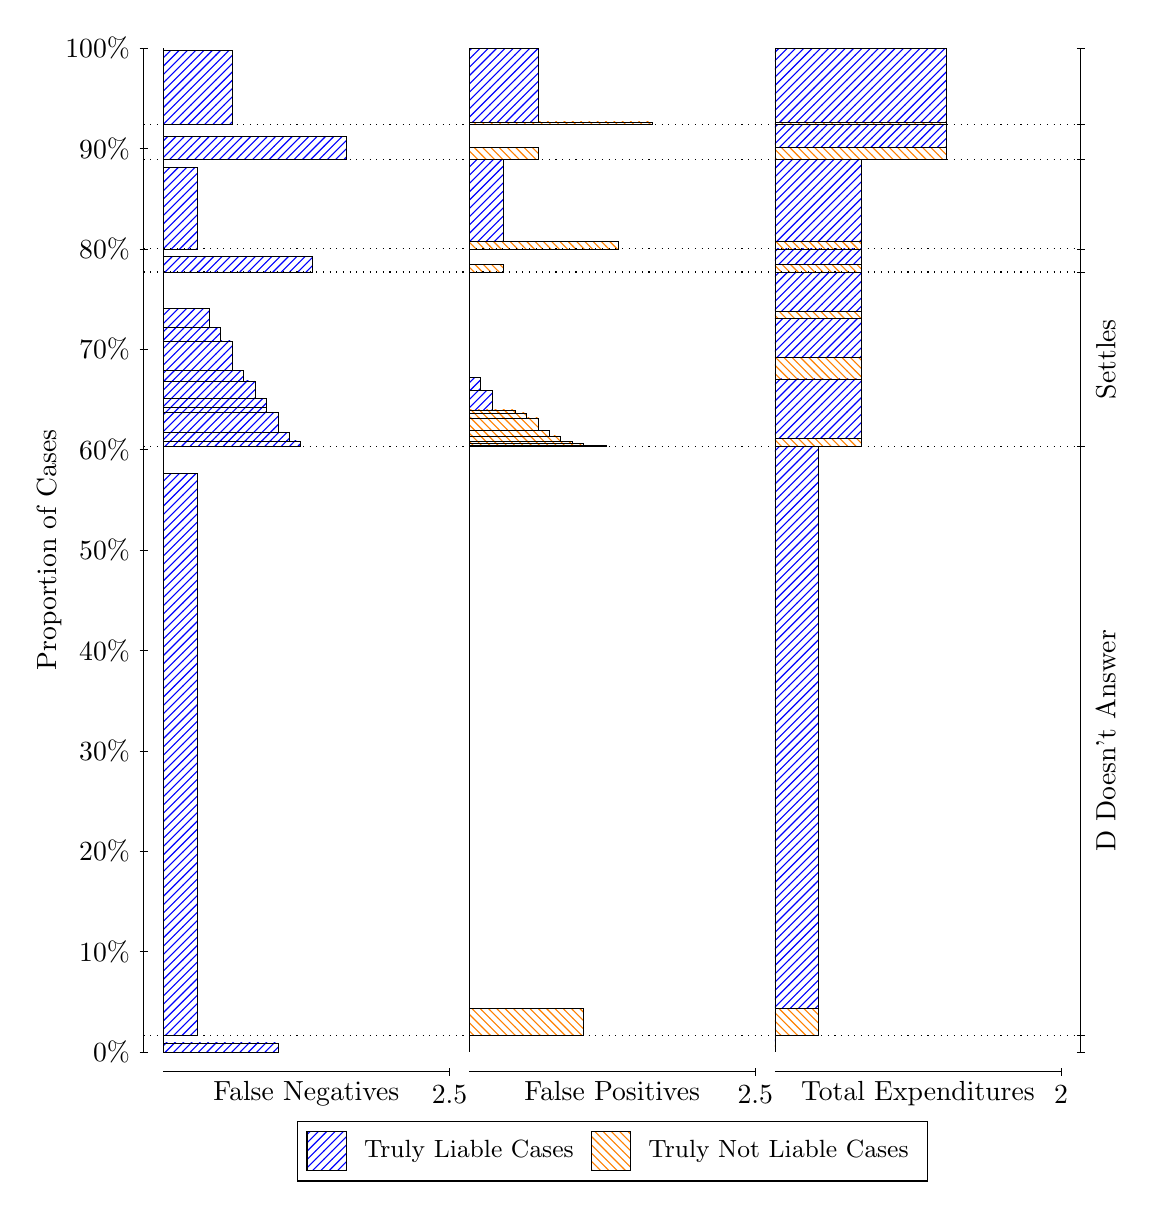
\begin{tikzpicture}
\draw[black, very thin] (1.5,1.75) -- (1.5,14.5);
\node[rotate=90, text=black, anchor=center] at (0.3, 8.125) {Proportion of Cases};
\draw[black, very thin] (1.45,1.75) -- (1.55,1.75);
\node[text=black, anchor=east] at (1.45, 1.75) {0\%};
\draw[black, very thin] (1.45,3.025) -- (1.55,3.025);
\node[text=black, anchor=east] at (1.45, 3.025) {10\%};
\draw[black, very thin] (1.45,4.3) -- (1.55,4.3);
\node[text=black, anchor=east] at (1.45, 4.3) {20\%};
\draw[black, very thin] (1.45,5.575) -- (1.55,5.575);
\node[text=black, anchor=east] at (1.45, 5.575) {30\%};
\draw[black, very thin] (1.45,6.85) -- (1.55,6.85);
\node[text=black, anchor=east] at (1.45, 6.85) {40\%};
\draw[black, very thin] (1.45,8.125) -- (1.55,8.125);
\node[text=black, anchor=east] at (1.45, 8.125) {50\%};
\draw[black, very thin] (1.45,9.4) -- (1.55,9.4);
\node[text=black, anchor=east] at (1.45, 9.4) {60\%};
\draw[black, very thin] (1.45,10.675) -- (1.55,10.675);
\node[text=black, anchor=east] at (1.45, 10.675) {70\%};
\draw[black, very thin] (1.45,11.95) -- (1.55,11.95);
\node[text=black, anchor=east] at (1.45, 11.95) {80\%};
\draw[black, very thin] (1.45,13.225) -- (1.55,13.225);
\node[text=black, anchor=east] at (1.45, 13.225) {90\%};
\draw[black, very thin] (1.45,14.5) -- (1.55,14.5);
\node[text=black, anchor=east] at (1.45, 14.5) {100\%};

\draw[black, very thin] (13.4,1.75) -- (13.4,14.5);
\draw[black, very thin] (13.35,1.75) -- (13.45,1.75);
\node[anchor=west] at (13.35, 1.75) {};
\draw[black, very thin] (13.35,1.9571) -- (13.45,1.9571);
\node[anchor=west] at (13.35, 1.9571) {};
\draw[black, very thin] (13.35,9.4422) -- (13.45,9.4422);
\node[anchor=west] at (13.35, 9.4422) {};
\draw[black, very thin] (13.35,11.655) -- (13.45,11.655);
\node[anchor=west] at (13.35, 11.655) {};
\draw[black, very thin] (13.35,11.95) -- (13.45,11.95);
\node[anchor=west] at (13.35, 11.95) {};
\draw[black, very thin] (13.35,13.085) -- (13.45,13.085);
\node[anchor=west] at (13.35, 13.085) {};
\draw[black, very thin] (13.35,13.529) -- (13.45,13.529);
\node[anchor=west] at (13.35, 13.529) {};
\draw[black, very thin] (13.35,14.5) -- (13.45,14.5);
\node[anchor=west] at (13.35, 14.5) {};

\draw[black, very thin, pattern color=blue, pattern=north east lines] (1.75,1.75) rectangle (3.2033,1.8654);
\draw[black, very thin, pattern color=orange, pattern=north west lines] (1.75,1.8654) rectangle (1.75,1.9571);
\draw[black, very thin, pattern color=blue, pattern=north east lines] (1.75,1.9571) rectangle (2.186,9.1002);
\draw[black, very thin, pattern color=orange, pattern=north west lines] (1.75,9.1002) rectangle (1.75,9.4422);
\draw[black, very thin, pattern color=blue, pattern=north east lines] (1.75,9.4422) rectangle (3.494,9.512);
\draw[black, very thin, pattern color=blue, pattern=north east lines] (1.75,9.512) rectangle (3.3487,9.6198);
\draw[black, very thin, pattern color=blue, pattern=north east lines] (1.75,9.6198) rectangle (3.2033,9.8726);
\draw[black, very thin, pattern color=blue, pattern=north east lines] (1.75,9.8726) rectangle (3.058,9.9374);
\draw[black, very thin, pattern color=blue, pattern=north east lines] (1.75,9.9374) rectangle (3.058,10.054);
\draw[black, very thin, pattern color=blue, pattern=north east lines] (1.75,10.054) rectangle (2.9127,10.274);
\draw[black, very thin, pattern color=blue, pattern=north east lines] (1.75,10.274) rectangle (2.7673,10.41);
\draw[black, very thin, pattern color=blue, pattern=north east lines] (1.75,10.41) rectangle (2.622,10.78);
\draw[black, very thin, pattern color=blue, pattern=north east lines] (1.75,10.78) rectangle (2.4767,10.949);
\draw[black, very thin, pattern color=blue, pattern=north east lines] (1.75,10.949) rectangle (2.3313,11.192);
\draw[black, very thin, pattern color=orange, pattern=north west lines] (1.75,11.192) rectangle (1.75,11.655);
\draw[black, very thin, pattern color=blue, pattern=north east lines] (1.75,11.655) rectangle (3.6393,11.854);
\draw[black, very thin, pattern color=orange, pattern=north west lines] (1.75,11.854) rectangle (1.75,11.95);
\draw[black, very thin, pattern color=blue, pattern=north east lines] (1.75,11.95) rectangle (2.186,12.985);
\draw[black, very thin, pattern color=orange, pattern=north west lines] (1.75,12.985) rectangle (1.75,13.085);
\draw[black, very thin, pattern color=blue, pattern=north east lines] (1.75,13.085) rectangle (4.0753,13.378);
\draw[black, very thin, pattern color=orange, pattern=north west lines] (1.75,13.378) rectangle (1.75,13.529);
\draw[black, very thin, pattern color=blue, pattern=north east lines] (1.75,13.529) rectangle (2.622,14.468);
\draw[black, very thin, pattern color=orange, pattern=north west lines] (1.75,14.468) rectangle (1.75,14.5);
\draw[black, very thin, pattern color=orange, pattern=north west lines] (5.6333,1.75) rectangle (5.6333,1.8417);
\draw[black, very thin, pattern color=blue, pattern=north east lines] (5.6333,1.8417) rectangle (5.6333,1.9571);
\draw[black, very thin, pattern color=orange, pattern=north west lines] (5.6333,1.9571) rectangle (7.0867,2.2991);
\draw[black, very thin, pattern color=blue, pattern=north east lines] (5.6333,2.2991) rectangle (5.6333,9.4422);
\draw[black, very thin, pattern color=orange, pattern=north west lines] (5.6333,9.4422) rectangle (7.3773,9.4503);
\draw[black, very thin, pattern color=orange, pattern=north west lines] (5.6333,9.4503) rectangle (7.232,9.4582);
\draw[black, very thin, pattern color=orange, pattern=north west lines] (5.6333,9.4582) rectangle (7.0867,9.481);
\draw[black, very thin, pattern color=orange, pattern=north west lines] (5.6333,9.481) rectangle (6.9413,9.5093);
\draw[black, very thin, pattern color=orange, pattern=north west lines] (5.6333,9.5093) rectangle (6.796,9.5751);
\draw[black, very thin, pattern color=orange, pattern=north west lines] (5.6333,9.5751) rectangle (6.6507,9.6489);
\draw[black, very thin, pattern color=orange, pattern=north west lines] (5.6333,9.6489) rectangle (6.5053,9.8015);
\draw[black, very thin, pattern color=orange, pattern=north west lines] (5.6333,9.8015) rectangle (6.36,9.8661);
\draw[black, very thin, pattern color=orange, pattern=north west lines] (5.6333,9.8661) rectangle (6.2147,9.9047);
\draw[black, very thin, pattern color=blue, pattern=north east lines] (5.6333,9.9047) rectangle (5.924,10.148);
\draw[black, very thin, pattern color=blue, pattern=north east lines] (5.6333,10.148) rectangle (5.7787,10.317);
\draw[black, very thin, pattern color=blue, pattern=north east lines] (5.6333,10.317) rectangle (5.6333,11.655);
\draw[black, very thin, pattern color=orange, pattern=north west lines] (5.6333,11.655) rectangle (6.0693,11.751);
\draw[black, very thin, pattern color=blue, pattern=north east lines] (5.6333,11.751) rectangle (5.6333,11.95);
\draw[black, very thin, pattern color=orange, pattern=north west lines] (5.6333,11.95) rectangle (7.5227,12.049);
\draw[black, very thin, pattern color=blue, pattern=north east lines] (5.6333,12.049) rectangle (6.0693,13.085);
\draw[black, very thin, pattern color=orange, pattern=north west lines] (5.6333,13.085) rectangle (6.5053,13.235);
\draw[black, very thin, pattern color=blue, pattern=north east lines] (5.6333,13.235) rectangle (5.6333,13.529);
\draw[black, very thin, pattern color=orange, pattern=north west lines] (5.6333,13.529) rectangle (7.9587,13.561);
\draw[black, very thin, pattern color=blue, pattern=north east lines] (5.6333,13.561) rectangle (6.5053,14.5);
\draw[black, very thin, pattern color=orange, pattern=north west lines] (9.5167,1.75) rectangle (9.5167,1.8417);
\draw[black, very thin, pattern color=blue, pattern=north east lines] (9.5167,1.8417) rectangle (9.5167,1.9571);
\draw[black, very thin, pattern color=orange, pattern=north west lines] (9.5167,1.9571) rectangle (10.062,2.2991);
\draw[black, very thin, pattern color=blue, pattern=north east lines] (9.5167,2.2991) rectangle (10.062,9.4422);
\draw[black, very thin, pattern color=orange, pattern=north west lines] (9.5167,9.4422) rectangle (10.607,9.5387);
\draw[black, very thin, pattern color=blue, pattern=north east lines] (9.5167,9.5387) rectangle (10.607,10.297);
\draw[black, very thin, pattern color=orange, pattern=north west lines] (9.5167,10.297) rectangle (10.607,10.567);
\draw[black, very thin, pattern color=blue, pattern=north east lines] (9.5167,10.567) rectangle (10.607,11.062);
\draw[black, very thin, pattern color=orange, pattern=north west lines] (9.5167,11.062) rectangle (10.607,11.159);
\draw[black, very thin, pattern color=blue, pattern=north east lines] (9.5167,11.159) rectangle (10.607,11.655);
\draw[black, very thin, pattern color=orange, pattern=north west lines] (9.5167,11.655) rectangle (10.607,11.751);
\draw[black, very thin, pattern color=blue, pattern=north east lines] (9.5167,11.751) rectangle (10.607,11.95);
\draw[black, very thin, pattern color=orange, pattern=north west lines] (9.5167,11.95) rectangle (10.607,12.049);
\draw[black, very thin, pattern color=blue, pattern=north east lines] (9.5167,12.049) rectangle (10.607,13.085);
\draw[black, very thin, pattern color=orange, pattern=north west lines] (9.5167,13.085) rectangle (11.697,13.235);
\draw[black, very thin, pattern color=blue, pattern=north east lines] (9.5167,13.235) rectangle (11.697,13.529);
\draw[black, very thin, pattern color=orange, pattern=north west lines] (9.5167,13.529) rectangle (11.697,13.561);
\draw[black, very thin, pattern color=blue, pattern=north east lines] (9.5167,13.561) rectangle (11.697,14.5);
\draw[black, dotted] (1.5,1.9571) -- (13.4,1.9571);
\draw[black, dotted] (1.5,9.4422) -- (13.4,9.4422);
\draw[black, dotted] (1.5,11.655) -- (13.4,11.655);
\draw[black, dotted] (1.5,11.95) -- (13.4,11.95);
\draw[black, dotted] (1.5,13.085) -- (13.4,13.085);
\draw[black, dotted] (1.5,13.529) -- (13.4,13.529);
\draw[black, very thin] (1.75,1.5) -- (5.3833,1.5);
\node[text=black, anchor=north] at (3.5667, 1.5) {False Negatives};
\draw[black, very thin] (5.3833,1.45) -- (5.3833,1.55);
\node[text=black, anchor=north] at (5.3833, 1.45) {2.5};

\draw[black, very thin] (5.6333,1.5) -- (9.2667,1.5);
\node[text=black, anchor=north] at (7.45, 1.5) {False Positives};
\draw[black, very thin] (9.2667,1.45) -- (9.2667,1.55);
\node[text=black, anchor=north] at (9.2667, 1.45) {2.5};

\draw[black, very thin] (9.5167,1.5) -- (13.15,1.5);
\node[text=black, anchor=north] at (11.333, 1.5) {Total Expenditures};
\draw[black, very thin] (13.15,1.45) -- (13.15,1.55);
\node[text=black, anchor=north] at (13.15, 1.45) {2};


\node[text=black, centered, rotate=90] at (13.72, 5.6996) {D Doesn't Answer};
\node[text=black, centered, rotate=90] at (13.72, 10.549) {Settles};





\draw (7.449999999999999,1.5) node[draw=none] (baseCoordinate) {};
\begin{scope}[align=center]
        \matrix[scale=0.5, draw=black, below=0.5cm of baseCoordinate, nodes={draw}, column sep=0.1cm]{
            \node[rectangle, draw, minimum width=0.5cm, minimum height=0.5cm, pattern color=blue, pattern=north east lines] {}; &
            \node[draw=none, font=\small, text=black] (B) {Truly Liable Cases}; &
            \node[rectangle, draw, minimum width=0.5cm, minimum height=0.5cm, pattern color=orange, pattern=north west lines] {}; &
            \node[draw=none, font=\small, text=black] (B) {Truly Not Liable Cases}; \\
            };
\end{scope}

\end{tikzpicture}
\end{document}